\newpage
\subsection{WP2 DAQ (8 pages)}
%{\bf Key deliverable:} Front- and back-end components of the DUNE far
%detector DAQ: Hardware, firmware and software for filtering,
%hit-finding and compression.  Software on COTS computers for reliable
%efficient movement of data and triggering.
%%This was new

%{\bf Strategic goals:} i) Continued UK intellectual leadership of the
%DUNE data acquisition (DAQ) system through the development and
%deployment of hardware, firmware and software parts and ii) maintain
%the UK in the position to lead the consortium of institutes
%contributing to construction of the far detector DAQ system.
%%This was edited from Pre-con grant

\subsubsection{Introduction}

The DUNE far detector data acquisition system is designed to exploit
the features of liquid argon technology for physics studies
in neutrino oscillations, rare decay searches and supernova neutrinos.
It is required to accept triggers from external sources (beam
interactions from Fermilab, calibration etc.), trigger internally
(atmospheric neutrinos, proton decay, solar neutrinos) and record data
over a period of a few milliseconds (corresponding to a drift time
window, or a part of it), for all, or a smaller group of APAs
surrounding the trigger.  In addition, the data acquisition must
robustly collect the full TPC waveform information on all the channels
over a period of tens of seconds should a supernova occur in our
galaxy and emit an intense burst of neutrinos.

Following developments in other HEP experiments, the DUNE DAQ is implemented
with a flexible combination of high-speed serial links, field-programmable
gate arrays (FPGAs) and computers.  It maximises the use of commercial
off-the-shelf (COTS) equipment, standardised around PCIe and Ethernet,
which allows us to procure the most modern equipment close to the installation
date and facilitates later upgrading.  In common with the strategy used by
other experiments, including the upgrades at the LHC, we have minimised the
number of designs of custom circuit boards, limited to two boards, one of 
which is to be designed and built in the UK, which are
used on all the sub-detector components.  The exact nature of the two
boards is still fluid as we are seeking to do parallel development with
LHC upgrade projects (although we are not reliant on them) to further increase
the maintainability and flexibility of the DAQ system.

The functional block diagram is shown in figure~\ref{fig:DAQBlock}(a).  There 
is a two-level trigger.  Level 1, which does most of the `heavy lifting', is 
implemented in a combination of FPGA and CPU.  To make it cost-effective, 
without reducing performance, the full data is retained in local buffers 
in the front-end data processing module (DPM) while a small subset
representing hits on the wires and photo-detectors is sent to a central
level~1 trigger processing farm; messages are then sent back to the local
buffers to retrieve the triggered portion of the full data.  The full
waveforms in the drift-time window of the triggers are then built into
events.  The level 2 data reduction is performed in software to remove
noise-generated events and to compress calibration.  The full output
of the detector is required to be less than 15PB/y and is composed of
the event types in table 1, reduced from an initial waveform raw data
rate of over 4TB/s.

\begin{figure}[tb]
    \centering
    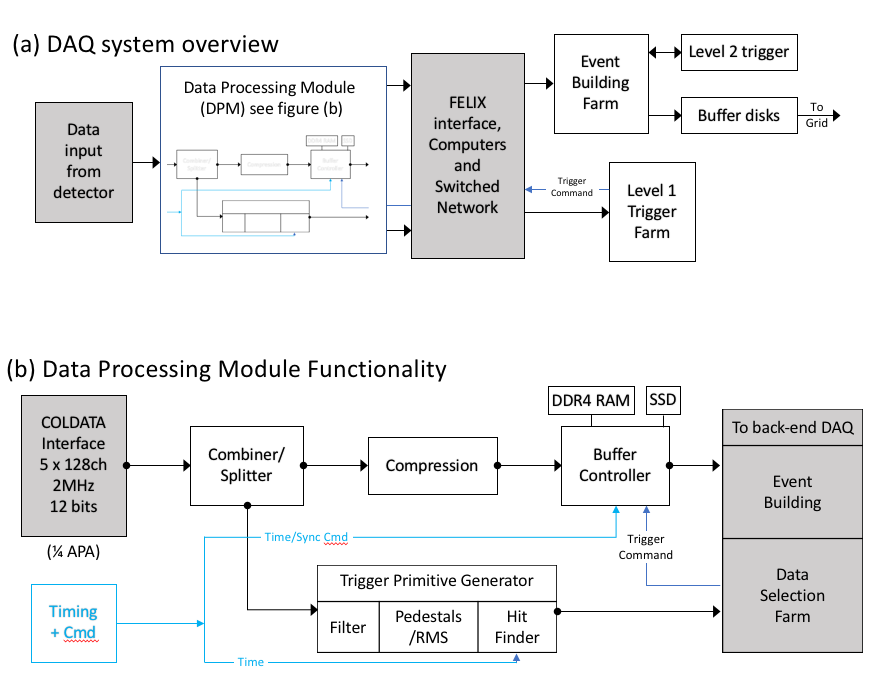
\includegraphics[width=0.98\textwidth]{figs/WP2/DAQBlockDiag.png}
    \caption{(a) Overview of the DAQ system (b) Detail of the data processing module.  The boxes in grey are not in the UK scope.  The scope of the event builder is shared with FNAL and the L1 trigger farm is shared with universities in the USA}
    \label{fig:DAQBlock}
\end{figure}

The largest challenge in the DAQ system is implementing algorithms
that can distinguish ionisation of interesting particle tracks from
signals due to electronic detector noise and from radioactive decays
of Argon-39 and other nuclei.  The signal-to-noise is expected to be
8 and 25 {\bf TODO: Get correct numbers} in the single- and
dual-phase TPCs respectively. The uncertainty in the levels and
characteristics of the noise in the single-phase TPC place strong
requirements to provide maximum flexibility in the filtering that precedes
the trigger hit-finding. This is the primary reason why the design 
is not completely fixed yet.   Although the DAQ is designed to be scalable,
to allow more processing to be added in parallel, this is limited
by the underground power (maximum 450kVA over all four modules).
We therefore provide the required flexible noise-filtering capability
using a combination of FPGAs (excellent power consumption per operation)
and CPUs (flexible, easy to combine non-local channels).

An important result of the simulation studies and architecture design we
have conducted is that at the front end, the processing steps in DUNE are
remarkably decoupled and can proceed in parallel without tricky
communication from channels to their neighbours. First individual hits 
on the collection planes are identified in the FPGAs, then associations of
hits on near-adjacent wires are performed in CPUs that are local to
each APA and finally clusters are associated together across the whole
module in the level~1 trigger farm, before the trigger requests are
returned to the local FPGAs to instruct retrieval of the full data.

The recent construction of smaller liquid argon detectors has been
crucial for experiencing the variation in the noise levels that can be
present in these detectors.  MicroBooNE followed a careful design
strategy and systematic identification and elimination of noise in the
commissioning phase, including noise at isolated frequencies
coherently induced on the wires from power regulators.  The 35t had
some similar and some different features, but overall the noise was 
much higher and highly-problematic.  The next iteration on the
electronics design, at ProtoDUNE has yielded a much quieter detector.
The likely noise in the far-detector is of the level of ProtoDUNE, but
to allow headroom, the DAQ design will be required to cope with noise
like that seen in MicroBooNE (with the thermal noise increased by the
longer wire-length in DUNE).  Should the noise exceed this in a way
that renders the provided trigger hardware ineffective, a provision is
made in a collaboration-held-risk (i.e. not in the DAQ) at additional
cost, to ship the data to the surface where a more elaborate signal
processing could be made in a large computer farm.

Figure~\ref{fig:DAQBlock}(b) shows a more detailed block diagram of the
DPM, which is the hardware module to be constructed in the UK.  The FPGA 
soft-logic will implement two pipelines to implement the front-end part 
of the full DAQ functionality as described above.

In the data storage pipeline, the main processing element is the
compression.  The data is first blocked to allow decompression to
start at predefined points and provide indexing.  Simple Fibonacci or
Huffman encoding schemes of the difference between successive samples
that don't use much FPGA fabric are under study.  These should reliably
compress to a factor of at least two, which is sufficient for DUNE.
More complex arithmetic encoding algorithms are in principle able to
obtain a factor of around four compression, but the trade-off between
extra processing or memory and bandwidth is less advantageous, so the
simpler approach is likely best.
These data are then multiplexed and 
written to a local DRAM memory buffer to wait for the trigger decision. 

In the trigger pipeline, a filtering stage is used to remove the high
frequency end of the noise spectrum and notch induced signals at fixed
frequencies.  Studies have shown finite-impulse-response (FIR) filters
to be effective against simulated noise with the MicroBooNE
specification.  The raw ADCs are digitised at 2\/MHz so multiplexing
many channels onto a pipeline allow a sufficient number of taps on the
filter in the reasonably priced FPGA we have selected.  Following
this, a pedestal subtraction algorithm and then hit finding (with
variable thresholds and disabling of excessively noisy channels) is
carried out, and the resulting hits made into a list for sending to
the CPU.

The supernova burst (SNB) handling in the DAQ is a challenging and
refreshingly novel requirement for a data acquisition system.  The principle 
SNB strategy for a large supernova in our galaxy, during which many thousand 
neutrino interactions are detected over a 10\/s period is provided by the
DRAM and solid state drive (SSD) devices on the DPM as shown in 
figure~\ref{fig:DAQBlock}. The central trigger will take a few seconds to accumulate
a larger-than-statistical fluctuation of SNB candidate interactions and will then
instruct the front-ends to spool all the raw compressed data from the DRAM to 
the SSDs on the front-end cards.  These data will later be read out (slowly).  
Four currently-available SSDs can store the data from a full APA at full 
speed in real-time, thus recording the data for many tens of seconds around such 
a trigger.  SSDs can't write continuously, however when combined with the DRAM 
and the trigger, they provide a suitable buffer; the DRAM allows several seconds 
prior to the SNB trigger to be recorded.

The resources requested in this grant cover the scope for the non-greyed boxes 
on figure~\ref{fig:DAQBlock}(a).  This covers hardware and computing needs for
two caverns, one implemented as a single-phase (APA readout) detector and 
the other using the dual phase-design, and also system software that can be 
used for all four caverns.  This comprises an in-house hardware component for
the front-end DAQ for the single-phase detector module only (WP2.1), computing 
equipment and software for the back end event building, level~1 and level~2 
trigger farms (WP2.2), the timing distribution system (WP2.3), and effort 
for installation (WP2.4), simulation, monitoring (WP2.5) and commissioning of
the first two modules.   Scope not contained in this grant request covers a 
middle layer of data transport, called FELIX, which moves data into a set 
of computers, and also, we will be assisted by international collaborators on
the back-end, installation and commissioning efforts.

It is certain the first cavern is single-phase, and the plan in this request
will adapt if the second cavern also uses the single-phase design, a decision 
is expected from the collaboration before mid-2019.

\subsubsection{Work plan}

The cost-optimised designs we are developing in the pre-construction
grant will be adapted to the final interfacing requirements of the
neighbouring parts of DUNE and the DAQ contributions from non-UK 
collaborators and a final pre-production prototype of the data 
processing module (DPM) will be made.  

The main challenges in the production and commissioning phase will 
be as follows:
\begin{itemize}
\item The production, testing and burn-in of the DPM cards for the
  single-phase cavern.  This is the one non-COTS component supplied by 
  the UK.
\item Software simulations, algorithms, utilisation and management to
  allow a robust and smooth flow of data through the back-end elements
  of the DAQ including trigger decision making, event building,
  run-control, monitoring, error handling and preparing data for
  archival.
\item Commissioning and tuning of the experiment to bring into
  operation all of the key functions to realise the physics goals of DUNE.
\end{itemize}

The planned activities build on the experience gained in operating the 
ProtoDUNE detector, starting in late-summer 2018 and on studies done and ongoing
to evaluate high-utilisation of CPU algorithms (SIMD instructions),
graphical processor units, design of error-resistant data transfer
(escalator protocol) and physics simulations of trigger algorithms.
We have also used a prototype of the timing distribution system on ProtoDUNE
and are developing the UK prototype of the DPM module.

\subsubsection{WP2.0 Overall management}

The management for the project will be provided jointly by Barr (40\%FTE 
on project) and Peeters (xx\%FTE on the project).  Cussans (xx\%FTE on 
project is the project engineer).  At the international level, Newbold 
is consortium leader.  Both Barr and Cussans have roles on the consortium 
management board and are co-conveners of the architecture and DAQ 
hardware subgroups respectively.

To maintain the excellent communication between international partners in the 
DUNE DAQ consortium, emphasis will be placed on giving status and summary talks
at the general consortium meetings and/or at specialised meetings of the 
consortium.  A UK-specific meeting, chaired by the project managers or the 
project engineer will be held weekly to discuss progress on the scheduled 
activities, plans for up-coming activities and to ensure that status
reports are given regularly to the consortium.

\subsubsection{WP2.1 Front-end trigger and data buffering module (DPM)}

The main way to handle the 1TB/s of digitised waveforms from each cavern 
is by feeding them through the custom processing pipelines implemented 
in FPGAs on UK-supplied boards.  The principle goals of the processing is to
distinguish the hits of ionising particles from electronics noise, and
coherent pickup which will hopefully be in localised parts of the
frequency domain.  We have a solid strategy for dealing with the known
sources of noise, but as experience shows from previous underground
experiments, the flexibility built into the system must be maximised
to allow removal of unexpected forms of high-rate background and to
allow innovative new approaches to triggering and compression to be
handled.  This is accomplished by using FPGAs in combination with 
downstream CPUs,  The layout that allows larger or smaller FPGAs to 
be used on the same board design to push this crucial choice later 
in the design cycle.  Extra parallelism can also be added by doubling-up 
the boards (which doesn't add as much electrical power consumption 
as additional CPUs would).  The design also allows high-throughput 
data transfer of all the data to the APA-level CPUs in the FELIX 
system for additional flexibility if the noise is considerably higher 
than specified.

The requirements, specification of the functional blocks and firmware
implementation are clear.  There is a possible value-engineering step
with the hardware that will be studied for the TDR, once the ProtoDUNE
preparation is completed.  The design that is described and costed
here involves mounting the DPM on its own PCB in its own crate.  The
optimisation, which is unlikely to change the cost to the UK much, but
might increase the integration is to redesign the FELIX card which
contains its own Kintex FPGA to be more closely integrated with the
DPM, either by combining onto one PCIe board, or by combining into a
single FPGA with the DRAM memory and SSDs attached.  It depends
whether the FELIX card will be redesigned anyway to obtain the newer
generation of PCIe logic available on the latest Xilinx Kintex
Ultrascale+ devices.

\subsubsection*{WP2.1.1 FPGA board management}

To facilitate the progression of the development of the project, 
the management is broken down into two interleaved hierarchies.  
The main WBS hierarchy is to coordinate specialist expertise 
(hardware, firmware, software etc.) as described in the WBS 
sections below.  Crossing this structure is a hierarchy of 
focused missions to implement a particular step in the
DAQ delivery.  These delivery coordination (DC) steps are outlined here

\paragraph{DC\/1 Delivery of production prototype DPM board} Coordinator: ?

\noindent
This step in the project is to take the prototypes from the 
pre-construction phase, and the decisions and outcomes from 
the TDR and deliver the final prototype board, executed by a 
viable company for placing the large contract.  It includes 
interfacing the firmware and hardware parts together (e.g. the 
constraints file).  

\paragraph{DC\/2 Mass-produce DPM board} Coordinator: Someone from RAL or IC?

\noindent
This step starts in parallel with DC\/1 above, it involves mapping out 
and obtaining approval for the tendering procedures.  The manager will 
explore whether to separate or combine the construction and loading of 
boards in one or more companies, and will communicate restrictions in 
capabilities (e.g.\ numbers of layers or small component placement) 
to the WP2.1.2 design team.

\paragraph{DC\/3 Functional implementation and QA} Coordinator: Someone with high FTE?

\noindent
Quality assurance (QA), verifying that the design and implementation will do
the job that is required of them is recognised as critical to the delivery 
of the DAQ project.  To ensure that it remains close to the physics, this 
task will include specification of the board functions and requirements, 
coordinating the design for the test setups.  It also includes specifying 
and organising writing the firmware and software suites for testing the 
boards, providing a user interface for using the boards in other test 
labs (e.g. for APAs, upstream-electronics or on-site during installation) and implementing the physics hit-finding/filtering/compression algorithms in the firmware infrastructure developed in WP2.1.3.  This last coordination task is to emphasise
the importance of the QA by linking it with the central physics functionality.

\paragraph{DC\/4 QC} Coordinator: ?

\noindent
Quality control (QC), verifying that each of the many boards constructed all
pass tests to certify they work as well as the first few that were used 
in the QA procedure outlined in DC\/3 above.  This involves designing 
and implementing a unit test workflow and possibly (if decided) installing 
it at the manufacturer for in-situ testing.  

\paragraph{WP2.1.2 Hardware} Manager: ?

\noindent
A prototype DPM, based on the SLAC RCE/COB architecture, and co-developed 
by Oxford and SLAC is approaching submission readiness.  This has given 
the project a head-start in high-speed board design involving DDR4 memory 
and 10Gb/s transmission.  Additionally, both RAL and Imperial have recently 
joined the project, with experience of design and construction of boards 
of similar or higher complexity for the CMS and ATLAS triggers.

During the remainder of the pre-construction project, the prototype DPM will
be completed, a test carrier board will be constructed and used for 
demonstration tests before the TDR.   Once the TDR architecture decisions 
have been made, and funding of the international partners is secured, the 
final iteration of design optimisation will be made, the decision of the final
form-factor of the board and its enclosure or crate will be made and the final
production-ready prototype of the DPM will be constructed (see DC\/1 above).

Paragraph with names from spreadsheet.

\paragraph{WP2.1.3 Firmware} Manager: ?
%The storage features described above are done with DRAM and SSDs
%attached to the FPGAs.  The writing of the DRAM buffer is done
%continuously using a write-pointer at the fixed incoming data rate.
%Two methods of organising the reading of the RAM buffer have been
%identified, in one, a processor on a Zynq Xilinx supplies the list of
%descriptors for the read locations to the logic.  In the other, the
%reads occur a fixed time after the writes and are matched with a
%time-ordered list of trigger requests provided by the CPU.

\noindent
There is considerable expertise in firmware development at Bristol, 
Imperial, Oxford, RAL and UCL.   The tasks in this work package are to 
supply firmware for testing the hardware and the various aspects of the 
design.   In parallel the firmware framework (in terms of top-level VHDL 
entity definitions) will be devised, sample algorithms will be written
and tests will be made with core FPGA IP to use the embedded interfaces on 
the chosen FPGAs (memory interfaces, PCIe interface, Ethernet etc.).
Most likely Xilinx will be the chosen type of FPGAs, but this has not 
been finalised yet.   

A crucial role in the firmware package is the management 
of the firmware source code repository, including code librarian, 
version management and ensuring regression tests are run on releases 
of our code and underlying packages (e.g. Vivado). 

The interface between the firmware and the control-software is a 
critical part of the project.  The coordination provided by DC\/1 
(see WP2.1.1 above) will drive the standardisation of this interface 
for the prototype project.  There is plenty of expertise in this area; 
two candidate frameworks that we can work from are (a) the CMS 
trigger code-base and (b) the SLAC Zynq-based system.  

Paragraph with names from spreadsheet.

\paragraph{WP2.1.4 Control software} Manager: ?

\noindent
The careful design and parallel implementation of control software 
alongside the firmware is crucial to the success of the project.  
The \texttt{pdtsbutler} concept developed by RAL and used in 
combination with the \texttt{BoardReader} interface to artDAQ for 
the timing system on ProtoDUNE is the model that we want to follow.  
It involves a standalone command-line driven interface to test all 
the low-level functions on the board, and available to the firmware 
authors.  The interface is also used to build up the more complex 
functions needed to configure and control the firmware during a physics 
run.  Finally a callable-interface to these functions is made and 
used in the \texttt{BoardReader} software.   This strategy has proved 
effective for allowing concurrent revisions of the firmware and 
different levels of software.

Paragraph with names from spreadsheet.

\paragraph{WP2.1.5 Photon detector and dual phase-detector interfaces} Manager ?

\noindent
blah

\paragraph{WP2.1.6 Optical links, installation and commissioning} Manager ?

\noindent
blah

\subsubsection{WP2.2 Back-end Event-Building}



\subsubsection*{WP2.2.1 Management}

\noindent
blah

\subsubsection*{WP2.2.2 Real-time transfers of trigger info with L1 farm}

\noindent
blah

\subsubsection*{WP2.2.3 Data transfers, event building and error handling}

\noindent
blah

\paragraph{WP2.2.4 COTS Procurement} Manager: G. Barr and someone at RAL?

\noindent
blah

\subsubsection*{WP2.2.5 Commissioning}

\noindent
blah

\subsubsection{WP2.3 Timing system}

\subsubsection{WP2.4 Facilities, Installation and Operations}

The installation of the four caverns of DUNE is complex involving many
interleaving sub-systems and schedules to address the challenges of
the detector location 4850ft underground.  It is therefore managed
centrally by the host-laboratories, financed through a common fund.
It is the UK plan to link closely to this and to supply in-kind
engineering effort to offset our common fund liability.  This will be
in the form of a dedicated person for 3s.y. and RAL TD effort for a
further $n$s.y., and much of the pre-installation work can be done from
the UK, with frequent phone and in-person meetings.  The installation
will be folllowed up with extensive effort from the other institutes,
for more DAQ specific tasks (some of which may not count towards
in-kind contributions, to be negotiated).

We have included the following resources into the current cost estimates
some of which should be eligible as in-kind CF contribution.

An assumption we have made that might be false is that we have costed the racks for each cavern separately, but it may be required to fit out the entire control room in one go including caverns 3 and 4.  I guessed that each rack would be a flat rate of GBP11k all inclusive (including things common to all racks such as power distribution etc.).  This is based on a quote from 2013 for a NEMA-12 rack with separate A/C unit (so not closely related to what we want) which was USD5k).

The milestones are closely tied to the collaboration-wide
organisation, and will move to the collaboration agreed dates when
they are known.

\subsubsection{WP2.5 Simulation and Performance Monitoring}

\subsubsection{Deliverables and Milestones}

Need advice on how much detail is needed in this section.  For now I dump in a few milestones from WP2.1.2 and WP2.4.  Should we just describe a few here, put the major milestones/deliverables in the appendix and leave the full list to the schedule?  If we want to put milestones in the text, we should define a \LaTeX macro to standardise.

\begin{tabular}{lp{12cm}}
M2.1.1  & preTDR decision on form-factor of DPM \\
M2.1.2  & Final specification of external interfaces for DPM, at TDR\\
M2.1.3  & Test of full firmware chain emulated on development board, and routed on
          full board design (yes, firmware before the board layout complete)\\
M2.1.4  & Schematic and board layout of integrated DPM\\
M2.1.5  & Prototype (allow one respin) DPM tested\\
M2.1.6  & Small production of protoyoype boards for test stands and possibly electronics and APA QC\\
M2.1.6  & Vertical slice test with integrated DPM, firmware and FELIX card (depends on FELIX firmware)\\
M2.1.7  & Prototype of QA testing firmware and computer software complete\\
M2.1.8  & Commercial tendering procedures for DPM production prepared\\
M2.1.9  & Commercial tendering procedures for DPM complete, contract awarded\\
M2.1.10 & Long-lead time components ordered\\
M2.1.11 & Final QA system delivered to manufacturer\\
M2.1.12 & Final production board design complete, ready for manufacturer to prototype\\
M2.1.13 & Production complete\\
M2.1.14 & In-house board testing complete\\
M2.1.15 & DPMs shipped to USA\\
M2.1.16 & Production boards used on vertical slice at CERN\\
M2.1.17 & Integration between DPM firmware/control SW and vertical slice run-control at CERN\\
M2.1.18 & DPMs arrive and clear customs in USA\\
M2.1.19 & DPMs installed at SURF\\
M2.1.20 & Integration between DPM firmware/control SW and vertical slice run-control at SURF\\
M2.1.21 & Pre-APA-installation release of firmware and control software\\
M2.1.22 & Use of DPMs as part of APA-installation cavern\\
M2.1.23 & Integration of firmware and control software with backend complete, configuration and monitoring functions complete\\
M2.1.24 & Pre-fill release of firmware and control software\\
M2.1.25 & Post-LAr fill release of firmware and control software (noise tuneup, monitoring tuneup) complete\\
M2.1.26 & Maintenance release of firmware and control software complete\\
\end{tabular}

\begin{tabular}{lp{12cm}}
M2.4.1 & Plan installation timeline and constraints \\
M2.4.2 & Installation related interfaces\\
M2.4.3 & Design the DAQ related plant e.g.\ Fibre bundles in caverns
         (SP design and DP design), Cable trays, Rack locations,
         sizes, power distribution, cooling\\
M2.4.4 & Rack procurement (potential UK supplier)\\
M2.4.5 & $\ldots$\\
\end{tabular}


\subsubsection{Business Case}
\newpage